\section{Jazyk}
\subsection{Premenné a pamäť}
K interpretácií algoritmu patria neoddeliteľne aj premenné, do ktorých algoritmus zapisuje, Máloktorý algoritmus sa zaoite bez jedinej premenej, napríklad true alebo false. Ako bolo povedané, tieto premenné sú definované jedinečnou kombináciou písmen, čísel a podržitiek. Samotné meno ale ešte negarantuje miesto kde sa bude dať zapisovať. Teda toto miesto sa musí najskôr prideliť tejto premenej. Pridelenie miesta je úlohou pamäti. 
Pamäť predstavuje miesto, kde sa dajú zapísať data. Dáta v jazyku Codewars predstavujú teda integer, real a Object. Funguje to tak, že pokiaľ si premenna N zažiada o miesto veľkosti M jednotiek, pamäť vyhľadá toľko jednoiek a označí ich ako obsadené. Zaujímavá situácia nastane, pokiaľ pamäť nemá dostupných toľko jednotiek. Existuje niekoľko možností, ako sa s tým vyrovnať. Jedna z nich je napríklad skutočne vráti už obsadené miesto a znehodnotiť tak zápisy, ktoré spravili iné premenné, alebo vytvpriť si jedno špeciálne miesto, ktoré bude čiernou dierov pre zápisy. To jest na premenné,na ktoré nevyšlo miesto, dostanú miesto na zápis v čiernej diere a nemôžu si byť ist že tam zápis zostane aj po ďalšom kole.
\subsection{rozdelenie a časti}
Pre aplikáciu bol vytvorený vlastný jazyk pomocou parsovacích nástrojov Flex a Bison z dôvodu ľahkej údržby a rozdelenia kódu na malé, ďalej nedeliteľné časti. Užívateľ teda bude mať veľmi detailný náhľad na to, ako algoritmus pracuje vnútri. Najmenšie pozorovateľné kúsky nazvime inštrukcie.\\
Vytvorený jazyk je syntaxou podobný jazyku PHP. Volba syntaxe vychádzala z toho že PHP je najrozšírenejšijazyk známu aj mimo infrmatickej sekcie a teda používateľny širšou masou. čo sa ale fungovania týka, musel byť upravený pre potreby aplikácie Codewars. Od PHP sa líši nasledujúcimi úpravami:
\begin{itemize}
\item na rozdiel od PHP jazyk Codewars nie je objektovo orientovaný nepodoporuje dedičnosť. Rozhodnutie o tejto vlastnosti vyplýva z technickej náročnosti implementovania dedičnosti a neznáme pojmy dedičnosť u širšej verejnosti
\item typy premenných museli byť tiež prispôsobené aplikácií Codewars. Preto jazyk podporuje iba premenné typu integer (celé 32-bitové číslo) a real, (je 4-bytové  číslo s plávajúcou desatinou čiarkou a so 7 významnými číslami). Naviac ale kvôli objektom na mape a robotom musí obsahovať novú premenú typu Location, ktorá bude definovať miesto na mape, a premennú typu Object, ktorá bude reprezentovať objekt na mape.
\item na rozdiel of PHP je nutné definovať typ premennej. K tomuto rozhodnutie vidla práve netrasparetnosť premenných, ku ktorým sa dá pristupovať ako k rôznym typom. Užívateľa prestane mať o danej premennej prehľad a tým sa hromadia napísané chyby, čo nie je účeom codewars.
\item jazyk nepotrebuje žiadne dodatočné knižnice ani funkcie. Musí byť však obohatený o funkcie pracujúce s premennými typu Object.
\item v jazyku nie je možné jak definovať nové štruktúry. Je však povolené vytvárať polia. K tomuto rozhodnutiu prispela zvlášť skutočnosť, že je jazyk obmedzený na tak málo typov a súčasne nie je podporená dedičnosť, kde sa nové štruktúry obzvlášť využívajú 
\end{itemize}
Z toho je vidno, že jazyk Codewars je oklieštený, ale zároveň rozšíriteľný o ďalšie funkcie a možnosti, ako napríklad používanie štruktúr. To sa napríklad rozšíri jeducho tak, že a pridá nové pravidlo na definovanie štruktúry, upraví pravidlo o výzore premennej a upraví spôsob, akým sa táto premenná bud ukladať.% nema to ist do impl?
\begin{itemize}
\item inicializovanie premennej, teda priradiť premennej miesto v pamäti. Je možné tento krok ešte malinko zobecnit na inštrukcie pre inicializovaie každej jednej položky, ako je to v Mlaskale, ale tento prístup len zbytočne zamlžuje informáciu, že savytvorila premenná daného mena.
\item inštrukcie pre nahranie premennej do zásobníka, odkiaľ sa neskôr použije jej hodnota. Premenná je definovaná svojím menom, čo je zhluk písmen alebo podržítka nezačínajúci číslovkou. Na túto inštrukciu sa dá nahliadať viacerými spôsobmi v závislosti na tom, ako vyzerá celkový mechaizmus spracovania jej hodnôt. Napríklad v jazyku Mlaska má táto inštrukcia niekoľko variant v závislosti na tom, či je premenná globálna, lokálna, a na jej type. Je to spôsobené rozdielnym chovaním v závislosti na tom, kde bola premenná definovaná a spôsobe, akým sa ukladajú hodnoty na vrchol zásobníka. Druhým spôsobom nazerania na túto inštrukciu je mať premenné všetky jedného typu a tie ukladať a zásobník, teda nie len hodnoty, ktoré sa buu zpracovávať, ale všetky, aké sú povolené. Táto metóda má zrejmú nevýhodu v zbytočnej veľkosti tejto premennej, avšak umožňuje napríklad pri prístupe na zlý typ okamžite zareagovať bez ejakého nepríjemného vedľajšieho efektu.
\item inštrukcie pre uloženie premenej. Vzhľadom a to, že na zásobníku budeme mať premennú všetkých typov, je vhodné si rozdeliť inštrukcie na uloženie každého jedného typu, Nastáva otázka, ako to je potom s uložením zloženého typu, napríklad poľa. Pole je v tom prípade nutné rozložiť na jednotlivé elemety a na na aplikovať inštrukcie o ukladaní premených jednoduchých typov. Tento prístup je podobný, aký sa použil v Mlaskale.
\item inštrukcie  na zničenie naalokovaných premenných. Toto sa týka hlavne okamihu, keď skončí blok. Premenné v ňom deklarované prestanú existovať. Opäť sa použije stejný princíp ako pri vytváraní premenných. Táto verzia je veľmi zjednodušená Garbage collectoru, aký sa používa napríklad v Jave, kde sa o deštrukcii premennej rozhoduje až potom, co sa heuristicky pomocou kódu zistí, že sa premenná už nepoužije.
\item inštrukcie pre zničenie dočasne alokovaných premenných.a Toto je nutné pri funkciách, ktorú maju návratovú hodnotu. Môže sa stať, že za návratovou hodotou nejde žiadna inštrukcia pre uloženie, takže by premenná zostava vidieť v zásobiku. Preto je táto inštrukcia nutná. Opäť ale vďaka tomu, že nahranie premennej na zásobník pridá práve jeden prvok, postači jedna inštrukcia pre každú dočasne naalokovanú premennú
\item inštrukcia pre volanie funkcie
\item inštrukcie pre aritmetické a relačné operátory, pre podporu najtriviálnejších funkcií
\item inštrukcie pre začatie a ukončenie bloku kvôli neskorším deinicializáciam
\item inštrukcie pre funkcie pýtajúce sa na objekty v mape.
\item inštrukcie pre konverzie. Keďže ale v tomto jazyku je sú jediné dve premenné, ktoré sa dajú na seba skonvertovať, budú to iba ľ typy inštrukcií
\end{itemize}
Nevýhody takto implementovaného jazyka:
\begin{itemize}
\item vytvárani premených zloženého typu prebieha rovnako ako inicializácia zložených typov, čo nie je úplne zodpovedajúce. Na druhej strane, detailné rozpísanie každej štruktúry, ako je to v je trochu matúce.\\
\item definícia premenných ako union všetkých možných typov, zaberá neprimerané množstvo pamäte, pričom sa využije len jedna časť
\end{itemize}
%\subsection{Funkcie a preddefinovanou hodnotou parametru}
%zavedeniu funkcie s preddefinovanou hodnotou parametre má jediný, pomerne malý dôvod. V okamihu, keď sa robot a nejaký iný objekt sa naplánujú na rovnaký čas, ten, ktorý sa naplánoval skôr, skôr tiež príde na radu (jedna z podmienok fair-play). Ak však robot zavolá funkciu, ktorá má preddefinovaný parameter, po zavolaní sa ocitne pred robotom, aj keby mali rovnaké programy a začínali rovnaký čas. To môže tomuto robotovi priniesť isté výhody, pretože sa dostane na radu skôr s predstihom minimálne 3 tickov (1 za assign a 2 za loadovanie premenných). Za ten čas sa podla tabuľky dá spraviť inštrukcia STEP a teda sa napríklad efektívne vyhnúť strele. V skratke, čím skôr sa robot dostane na radu, tým je to pre neho výhodnejsie, lebo môže skôr reagovať na udalosť a predísť následkom a tým viac sa na radu vlastne dostane. Príklad: Strela S je naplánovaná na čas {\it s1}, robot R je po rozmýšľaní 10 tickov pred strelou strelou (predpokladáme, že zavolal funkciu s preddefinovaným parametrom a inak by bol naplánovaný maximálne 9 tickov pred S) Za ten čas sa môže 2x pohnúť, poťažne použiť inštrukciu see, zistit polohu strely a vystreliť jej smerom.
%\subsection{Životnosť premenných vnútri bloku - scoping}
%\indent Podobne ako v programovacích jazykoch C, Java , Delphi a pod., je použité statické zapúzdrovanie premennych. To znamená, že prístup k hodnotám, na ktorá odkazuj dané meno premennej, je len v bloku, kde bola funkcia deklarovaná a v žiadnom ďalšom podbloku premenná s rovnakým menom nesmie byť deklarovaná. Napríklad vo funkcií 
%$for (integer i = 0; i<10; i++)
%{
%	code;
%}$
%premennú i už nie je možné použiť mimo cyklu a naopak táto premenná nebola predtým deklarovaná v žiadnom v nadradených cykloch. Vo väčšine programovacích jazykoch je zapuzdrovanie ideálnou metódou na zprehľadnenie kódu tým, že pod premennou s rovnakým menom sa skrýva premenná rôzneho typu v rámci bloku. Typickým príkladom napríklad v jazyku C je \\$for (int\ i =0; i< 10; i++)$ \\ $ {//blabla}$ \\V našom prípade je ale situácia trochu zložitejšia. Ako bolo povedané v úvode, každá inštrukcia robota niečo stojí, rovnako inizializovanie novej premennej a jej deinicializovanie tiež, takže z tohoto hľadiska na tom robot iba tratí,čo je temer vždy nežiaduce. Dôvod pre zavedenie zapúzdrovania aj v tomto prípade je, ze v okamihu, keď robot použije takúto funkciu, má to dva efekty: \\
%		\begin{itemize}
%		\item v pamati bude mať pochopitelne o jednu premennú viac. Keďže pamať robota nie je neobmedzená a je uživateľom definovaná na úkor iných vlastnosti(napríklad odolnosti voči zbraniam), pri kóde typu:
%for (integer i = 0; i< 10; i++)
%{
%	code
%}
%fce1();
%fce2();
%fce3();
%..
%môže pri nepodoporovanom zapúzdrovaní robotovi dojsť pamať napriek tomu, ze ďalšie použitie premennej i sa už ďalej nevyskytuje. Pri nepodporovanom zapúzdrenía súčasne výskyte premennej po danom cykle by bolo stejne akoby bola premenná definovaná v nadradenom cykle, to znamená, že až na virtuálne uvoľnenie premennej z pamäti robota by penalizácia bola úplne rovnaká.
%\end{itemize}
%Z tohoto dôvodu je teda zapúzdrovanie povolené. \\

%Problém môže nastať v okamihu, keď sú povolené rovkako rekurzívne funkcie. V okamihu zavolania takejto funkcie, 

Výhodou takéhoto detailného rozloženia kódu je okrem vysokej transparentnosti aj možnosť priradiť jednotlivým inštrukciám hodnotu, takzvanú penalizáciu. V reálnych hrách by to zodpovedalo zdržaniu pred vykonaním akcie. Typickým príkladom je mág v dobrudružných hrách, ktorý podporuje svoju družinu kúzlami. Štandartne ale potrebuje istý čas na vyrieknutie kúzla.\\
Podľa tohoto prieskumu teda výsledné potrebné inštrukcie sú popísané v tabuľke \ref{tab:instrukcie}
\begin{center}
\begin{longtable}{|l|l|}
\caption[používané inštrukcie]{používaneé inštrukcie}
\label{tab:instrukcie}\\
\hline \hline \\[-2ex]
\multicolumn{1}{c}{\textbf{názov inštrukcie}} &
\multicolumn{1}{c}{\textbf{výsledok akcie}} \\[0.5ex] \hline
\\[-1.8ex]
\endfirsthead

\multicolumn{2}{c}{{\tablename} \thetable{} -- pokračovanie} \\[0.5ex]
\hline \hline \\[-2ex]
\multicolumn{1}{c}{\textbf{názov inštrukcie}} &
\multicolumn{1}{c}{\textbf{výsledok akcie}} \\[0.5ex]\hline
\\[-1.8ex]
\endhead
InstructionCreate&\\
InstructionLoad&\\
InstructionConversionToInt&\\
InstructionConversionToReal&\\
InstructionDuplicate&\\
InstructionStoreRef&\\
InstructionStoreInteger&\\
InstructionStoreReal&\\
InstructionStoreObject&\\
Call&\\
InstructionPop&\\
InstructionMustJump&\\
InstructionJump&\\
InstructionBreak&\\
InstructionContinue&\\
InstructionReturn&\\
InstructionRestore&\\
InstructionRemoveTemp&\\
InstructionPlusPlusInteger&\\
InstructionPlusPlusReal&\\
InstructionMinusMinusInteger&\\
InstructionMinusMinusReal&\\
InstructionPlus&\\
InstructionPlusInteger&\\
InstructionPlusReal&\\
InstructionMinusInteger&\\
InstructionMinusReal&\\
InstructionMultiplyInteger&\\
InstructionMultiplyReal&\\
InstructionDivideInteger&\\
InstructionDivideReal&\\
InstructionModulo&\\
InstructionBinaryAnd&\\
InstructionAnd&\\
InstructionBinaryOr&\\
InstructionOr&\\
InstructionBinaryNot&\\
InstructionNot&\\
InstructionGtInteger&\\
InstructionGtReal&\\
InstructionGeInteger&\\
InstructionGeReal&\\
InstructionEqualInteger&\\
InstructionEqualReal&\\
InstructionEqualObject&\\
InstructionNotEqual&\\
InstructionNotEqualInteger&\\
InstructionNotEqualReal&\\
InstructionNotEqualObject&\\
InstructionLtInteger&\\
InstructionLtReal&\\
InstructionLeInteger&\\
InstructionLeReal&\\
InstructionBegin&\\
InstructionEndBlock&\\
InstructionSee&\\
InstructionEye&\\
InstructionFetchState&\\
InstructionStep&\\
InstructionStepDefault&\\
InstructionWait&\\
InstructionShootAngle&\\
InstructionTurn&\\
InstructionTurnR&\\
InstructionTurnL&\\
InstructionHit&\\
InstructionIsPlayer&\\
InstructionIsWall&\\
InstructionIsMissille&\\
InstructionLocate&\\
InstructionIsMoving&\\
InstructionTarget&\\
InstructionSaveVariable&\\
InstructionLoadVariable&\\
InstructionDirection&\\
InstructionRandom&\\
\hline
\end{longtable}
\end{center}
\subsection{Penalizácia a plánovanie}
penalizácia je zatiaľ implementovaná globálne, čo nie je najvhodnesie, pretože to vylučuje možnoť mať testovacieho robota, na ktorom chceme nacvičit boj napríklad proti kuzelníkovi. Detailné zobrazenie plánovača je zobrazené na obrázku \ref{fig:sch}
\begin{figure}
\centering
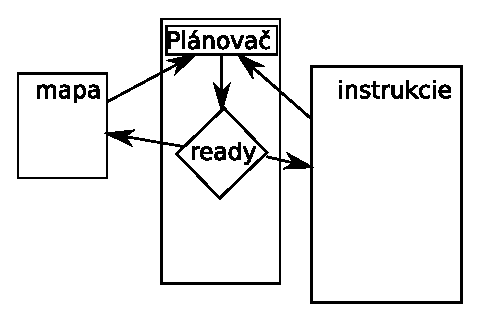
\includegraphics{planovac}
\caption{Chovanie plánovača}
\label{fig:sch}
\end{figure}
